\chapter{项目的财务评价}
\section{财务评价概述}
\subsection{财务评价的概念}
财务评价是根据国家现行的财税制度和价格体系,在财务效益与费用的估算以及编制财务辅助报表的基础上,\textbf{编制财务报表,计算财务分析指标,考察和分析项目的盈利能力、偿债能力和财务生存能力,判断项目的财务可行性},明确项目对财务主体的价值以及对投资者的贡献,为投资决策、融资决策以及银行贷款等提供依据。

  ——2006年国家发改委和建设部联合发布的《建设项目经济评价方法与参数》(第三版)

\subsection{财务评价的内容和步骤}
(1)选取财务评价基础数据与参数。

(2)估算财务效益与费用,形成财务评价辅助报表,编制资金规划与计划。

(3)编制财务评价的基本报表。

(4)根据融资前分析和融资后分析的要求,计算评价指标,进行盈利能力分析、偿债能力分析、财务生存能力分析等。

(5)不确定性分析和风险分析。

(6)形成财务评价结论。

\section{财务效益与费用估算}
\subsection{财务效益估算}
财务效益主要包括营业收入,项目得到的各种补贴、项目寿命期末回收的固定资产余值和流动资金。

营业收入包括销售产品或提供服务所获得的收入,其估算的基础数据,包括产品或服务的数量和价格。

对于生产多种产品和提供多项服务的,应分别估算各种产品及服务的营业收入。

\begin{figure}[H]
    \centering
    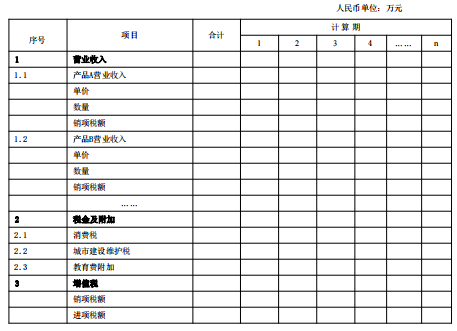
\includegraphics[width=1\linewidth]{image/营业收入、营业税金及附加和增值税估算表.png}
    \caption{营业收入、营业税金及附加和增值税估算表}
\end{figure}

\subsection{投资的估算}

\subsubsection{1. 建设投资估算}

\textbf{简单估算法、概算法、形成资产法}

项目规划和建议书阶段,投资估算要求精度低,可利用简单估算法。

单位生产能力法、生产能力指数法、系数估算法。

\noindent \textbf{A 单位生产能力法——简单估算法}

依据调查的统计资料,利用相近规模的单位生产能力投资乘以建设规模,即得拟建项目投资。

$$C_2=(\frac{C_1}{Q_1})Q_2f$$

式中,C1:已建类似项目的投资额;C2:拟建项目投资额;Q1:已建类似项目的生产能力;Q2:拟建项目的生产能力;f:不同时期、不同地点的定额、单价、费用变更等的综合调整系数。

\textbf{例:}假定某地拟建一座2000套客房的豪华旅馆,另有一座某豪华旅馆最近在该地竣工,且掌握了以下资料:它有2500套客房,有门厅、餐厅、会议室、游泳池、夜总会、网球场等设施。总造价为10250万美元。估算新建项目的总投资。

\textbf{解:}折算为每套客房的造价:4.1万美元

同一个地方,且各方面有可比性的具有2000套客房的豪华旅馆造价估算值为:4.1万美元×2000=8200万美元。

\noindent \textbf{B 生产能力指数法——简单估算法}

又称指数估算法,它是根据已建成的类似项目生产能力和投资额来粗略估算拟建项目投资额的方法,是对单位生产能力估算法的改进。
$$C_2=C_1(\frac{Q_2}{Q_1})^x \cdot f$$
式中:x—生产能力指数。正常情况下,$0 \leq x \leq 1$。

造价与规模(或容量)呈非线性关系,且单位造价随工程规模(或容量)的增大而减小。

\noindent \textbf{C 系数估算法——简单估算法}

以某个装置或某项设备费为基数,乘以适当系数来推算项目的建设费用。这种方法比较简单,但没有考虑设备规格、材质的差异,所以精确度不高。

总建设费用=主要设备费(1+管线、仪表、建筑等费用估算系数)*(1+间接费总估算系数)

\noindent \textbf{概算法和形成资产法}

按照费用的归集方式有概算法和形成资产法。

\textbf{概算法。}把建设项目划分为建筑工程费、设备购置费、安装工程费用及工程建设其他费用等费用项目或单位工程,再根据各种具体的投资估算指标,进行各项费用项目或单位工程投资的估算,在此基础上,可汇总成每一单项工程的投资。另外再估算工程建设其他费用及预备费,即求得项目建设总投资。

\textbf{形成资产法。}由形成固定资产的费用、形成无形资产的费用、形成其他资产的费用和预备费用四部分组成。

\noindent \textbf{建设投资的概算法}

\textbf{基本预备费估算:}是指在项目实施中可能发生难以预料的支出,需要事先预留的费用,又称工程不可预见费,主要指设计变更及施工过程中可能增加工程量的费用。基本预备费以建筑工程费、设备购置费、安装工程费及工程建设其他费用之和为计算基数乘以基本预备费率计算。

中石化:

(固定资产+无形资产+其他资产)$\times $不可预见费率

10\%-12\%,适用于综合类及国内无同类装置项目

8\%-10\%,适用于国内已见有同类装置项目。

\textbf{涨价预备费估算:}涨价预备费是对建设工期较长的项目,由于在建设期内可发生材料、设备、人工等价格上涨引起投资增加,需要事先预留的费用,也称价格变动不可预见费。涨价预备费以建筑工程费、设备购置费、安装工程费之和为计算基础。计算公式为:

$$PC=\sum_{i=1}^{n}I_t[(1+f)^t-1]$$

其中:PC—涨价预备费;$I_t$—第t年的建筑工程费、设备购置费和安装工程费之和;f—建设期价格上涨指数;n—建设期。

\subsubsection{2. 流动资金估算}

扩大指标估算法:是参照同类企业流动资金占营业收入或经营成本的比例、或者单位产量占用营运资金的数额估算流动资金。

在项目建议书阶段一般可采用扩大指标估算法。

流动资金=年营业收入额×营业收入资金率

流动资金=年经营成本×经营成本资金率

中石化石油天然气项目经营成本资金率:15\%-25\%

流动资金=年产量×单位产量占用流动资金额

\subsubsection{3. 建设期利息的估算}

建设期利息包括银行借款和其他债务资金的利息,以及其他融资费用。
其他融资费用是指某些债务融资中发生的手续费、承诺费、管理费、信贷保险费等融资费用。

通常假定借款均在每年的年中支用,借款当年按半年计算,其余各年份按全年计息。

各年应计利息=(年初借款本金累计+本年借款额/2)$\times $年利率

\subsection{总成本费用的估算}

\subsubsection{1. 生产成本加期间费用估算法}

即总成本费用=生产成本+期间费用

生产成本=直接材料费+直接燃料和动力费+直接工资+其他直接支出+制造费用

期间费用=管理费用+营业费用+财务费用

\subsubsection{2. 生产要素估算法}

总成本费用=外购原材料、燃料和动力费+工资及福利费+折旧费+摊销费+修理费+利息支出+其他费用

\subsection{经营成本的估算}

经营成本=外购原材料、燃料和动力费+工资及福利费+修理费+其他费用

如果以会计核算中的总成本费用为基础,则是在总成本费用中要扣除虽计入产品的成本费用中,但实际并没有发生现金支出的费用项目。

经营成本=总成本费用-折旧费-摊销费-利息支出

\subsection{税费的估算}

\textbf{增值税。}当采用含税价格计算销售收入和原材料、燃料动力成本时,利润和利润分配表以及现金流量表中应单列增值税科目;采用不含税价格计算时,利润和利润分配表以及现金流量表中不包含增值税科目。

\textbf{消费税。}我国对部分货物征收消费税。项目评价中对适用消费税的产品,应按税法规定计算消费税。

\textbf{土地增值税。}是按转让房地产取得的增值额征收的税种。房地产开发项目应按规定计算土地增值税。

\textbf{资源税。}是国家队开采特定矿产品或生产盐的单位和个人征收的税种。通常按矿产的产量计征。

在会计处理上,消费税、土地增值税、资源税和城建税、教育费附加均可包含在营业税金及附加中。税金及附加应作为利润和利润分配表中的科目。

\subsection{维持运营投资}

某些项目在运营期需要投入一定的固定资产投资才能得以维持正常运营,例如设备更新费用、矿山的井巷开拓延伸费用等。发生维持运营投资时应将其列入现金流量表作为现金流出,参与内部收益率的计算。同时,也应反映在财务计划现金流量表中,参与财务生存能力分析。

如煤炭项目,为维持正常生产,在生产期内需要投入一定的固定资产或费用,包括固定资产更新投资、安全生产投入、维简费开支的其他维持简单再生产投入、开拓延深费和追加投资等,这些维持运营投资,应在现金流量表中将其作为现金流出。

固定资产更新投资、开拓延深费和追加投资应予以资本化,安全生产投入、维检费开支等其他维持简单再生产投入应予以费用化。

\begin{figure}[H]
    \centering
    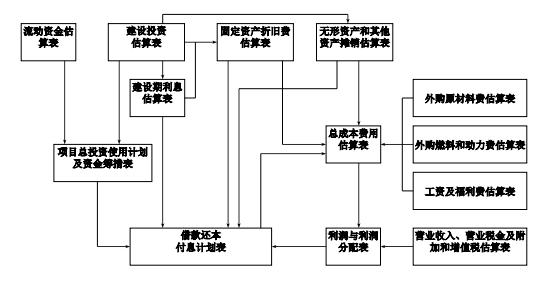
\includegraphics[width=\linewidth]{image/财务分析辅助报表关系图.png}
    \caption{财务分析辅助报表关系图}
\end{figure}

\section{财务评价的基本报表}

\noindent 复习要点:\\
\textbf{现金流量表 重点}\\
\textbf{1. 项目投资现金流量表 最重要}\\
\textbf{2. 项目资本金现金流量表 次重要}\\
\textbf{3. 投资各方现金流量表}\\
利润与利润分配表\\
财务计划现金流量表\\
借款还本付息计划表

\subsection{现金流量表}
\subsubsection{1.项目投资现金流量表(要求会编制)}
是以项目作为一个独立系统,不区分项目资金的来源,反映项目在整个计算期内的现金流入和现金流出,反映项目投资的盈利能力,用于计算项目投资内部收益率及净现值等财务分析指标。

其现金流量的计算与成本核算的算法不同,现金流量计算中只体现现金收支,不体现非现金的摊派(如折旧、摊销)等。

\begin{figure}[H]
    \centering
    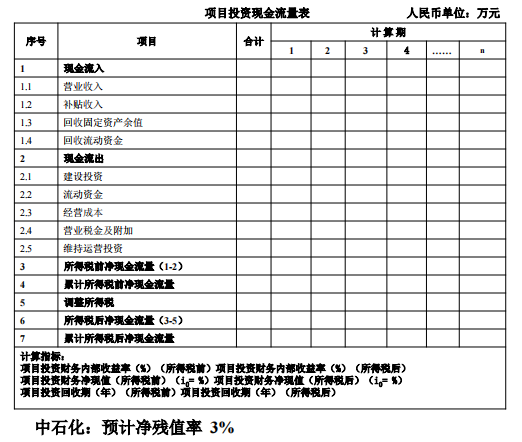
\includegraphics[width=0.6\linewidth]{image/项目投资现金流量表1.png}
    \caption{项目投资现金流量表}
\end{figure}

\subsubsection{2. 项目资本金现金流量表(不太重要)}
从项目法人(或投资者整体)角度出发,以项目资本金作为计算的基础,把借款本金偿还和利息支付作为现金流出,用以计算资本金内部收益率,反映投资者权益投资的获利能力。对资本金只计算税后净现金流量,因为税前净现金流量没有实际价值。

\begin{figure}[H]
    \centering
    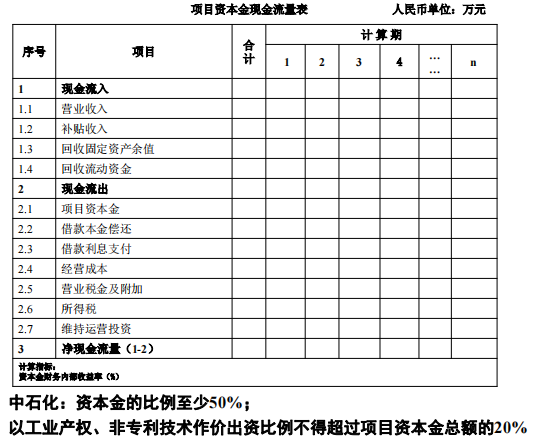
\includegraphics[width=0.6\linewidth]{image/项目资本金现金流量表.png}
    \caption{项目资本金现金流量表}
\end{figure}

\subsubsection{3. 投资各方现金流量表(自学)}
分别从各个投资者的角度出发,以投资者的出资额作为计算的基础,用于计算投资各方内部收益率。

\begin{figure}[H]
    \centering
    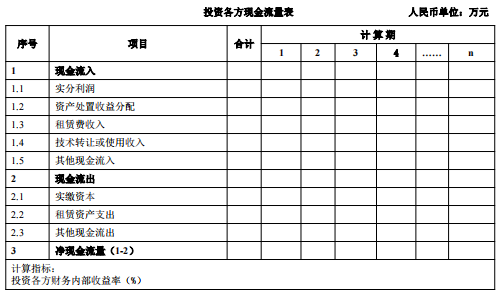
\includegraphics[width=0.6\linewidth]{image/投资各方现金流量表.png}
    \caption{投资各方现金流量表}
\end{figure}

\subsection{利润与利润分配表}
反映项目计算期内各年营业收入、总成本费用、利润总额等情况,以及所得税后利润的分配,用于计算总投资收益率、项目资本金净利润率等指标。

要求:会进行简单的利润计算。

利润=收入-总成本费用-营业税金及附加

掌握总成本费用与经营成本之间的区别与联系。

\begin{figure}[H]
    \centering
    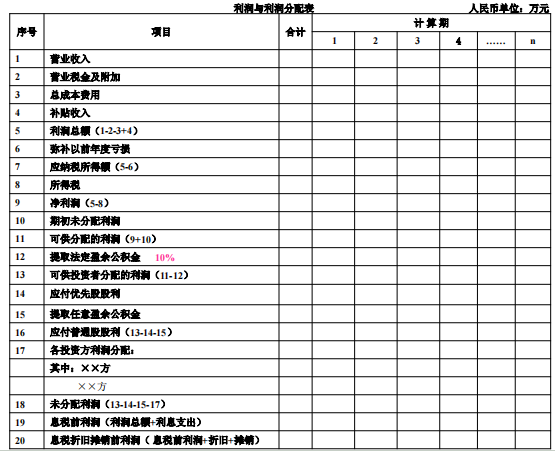
\includegraphics[width=0.6\linewidth]{image/利润与利润分配表.png}
    \caption{利润与利润分配表}
\end{figure}

\subsection{财务计划现金流量表(了解)}
反映项目计算期各年的投资、融资及经营活动的现金流入和流出,用于计算累计盈余资金,分析项目是否有足够的净现金流量维持正常运营,以实现财务可持续性,体现项目的财务生存能力。

\begin{figure}[H]
    \centering
    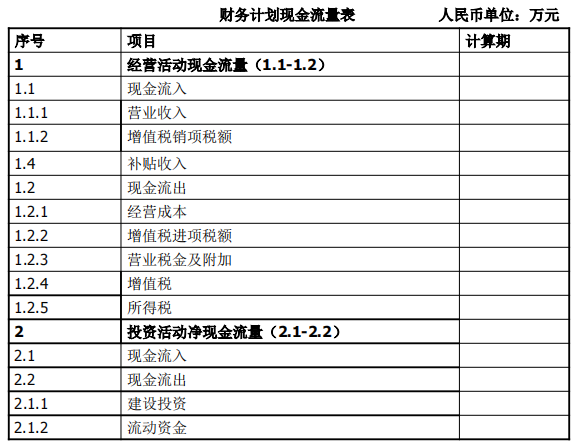
\includegraphics[width=0.6\linewidth]{image/财务计划现金流量表.png}
    \caption{财务计划现金流量表}
\end{figure}

\begin{figure}[H]
    \centering
    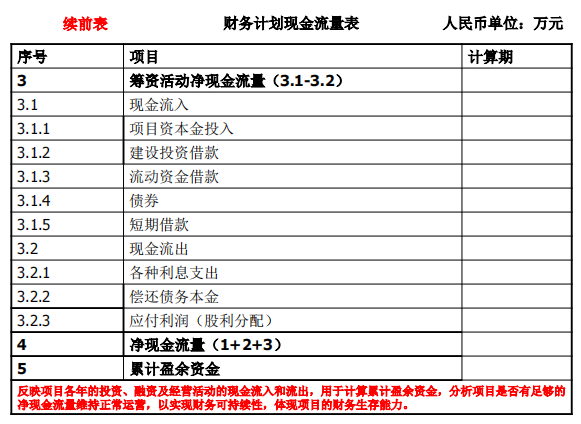
\includegraphics[width=0.6\linewidth]{image/财务计划现金流量表(续).png}
    \caption{财务计划现金流量表(续)}
\end{figure}

\section{财务评价的指标体系}
\subsection{盈利能力分析指标体系}
财务净现值、财务内部收益率、资本金财务内部收益率、投资各方财务内部收益率、项目动态投资回收期、总投资收益率、项目资本金净利润率、投资回收期。

\subsection{偿债能力指标体系}
\subsubsection{1. 利息备付率}
利息备付率= 税息前利润 / 当期应付利息 $\times$ 100\%

税息前利润=利润总额+计入总成本费用的利息费用;

当期应付利息—计入总成本费用中的应付利息。

利息备付率应分年计算,利息备付率高,表明利息偿付的保障程度高。

利息备付率应大于1,并结合债权人的要求确定。

\subsubsection{2. 偿债备付率}
偿债备付率=可用于还本付息的资金/当期应还本付息的金额 $\times $100\%

可用于还本付息的资金—包括可用于还款的折旧和摊销、成本中列支的利息费用、可用于还款的利润等,也即息税前利润加折旧和摊销;

应还本付息的金额—包括还本金额和计入总成本费用的全部利息。

偿债备付率应分年计算,偿债备付率高,表明可用于还本付息的资金保障程度高。

偿债备付率应大于1,并结合债权人的要求确定。

\subsubsection{3. 资产负债率}
资产负债率= 期末负债总额 / 期末资产总额 $\times $ 100\%

适度的资产负债率,表明企业经营安全、稳健,具有较强的筹资能力,也表明企业和债权人的风险较小。对该指标的分析,应结合国家宏观经济状况、行业发展趋势、企业所处竞争环境等具体条件判定。项目财务分析中,在长期债务还清后,可不再计算资产负债率。

\subsection{财务生存能力分析}
财务生存能力分析也称为资金平衡分析

拥有足够的经营净现金流量是财务可持续性的基本条件,特别是在运营初期。

各年累计盈余资金不出现负值是财务生存的必要条件。

\begin{figure}[H]
    \centering
    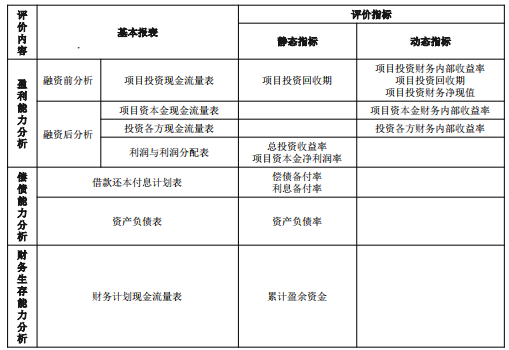
\includegraphics[width=0.6\linewidth]{image/财务分析和评价指标与基本财务报表的对应关系.png}
    \caption{财务分析和评价指标与基本财务报表的对应关系}
\end{figure}

\textbf{举例(重要,理解并掌握):}某项目总投资1350万元,其中固定资产投资1000万元,流动资金350万元,于项目第一年年初投入。项目当年建成投产,生产期10年,每年产品销售收入800万元,年经营成本400万元,年营业税金及附加80万元。固定资产投资全部形成固定资产原值,在生产期采用直线折旧法进行折旧,折旧年限为10年,净残值率为5\%。设所得税税率为40\%。

\begin{figure}[H]
    \centering
    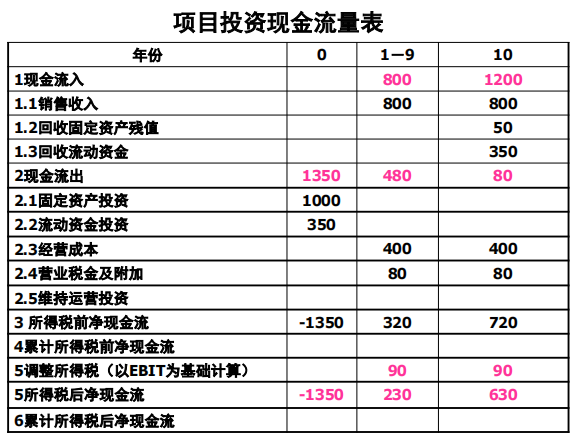
\includegraphics[width=0.6\linewidth]{image/项目投资现金流量表2.png}
\end{figure}

\textbf{例(续):}上述项目中固定资产投资中50\%是长期借款,年利率8\%,借款本金从生产期开始分10年等额偿还,每年支付未偿还借款的利息;流动资金投资的40\%来自借款,借款利率为5\%,第10年末一次偿还流动资金借款,每年支付相应利息。

\begin{figure}[H]
    \centering
    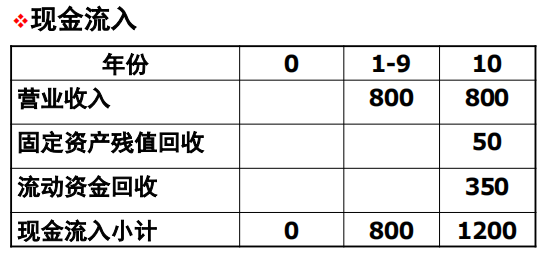
\includegraphics[width=0.75\linewidth]{image/生存能力分析1.png}
\end{figure}

\begin{figure}[H]
    \centering
    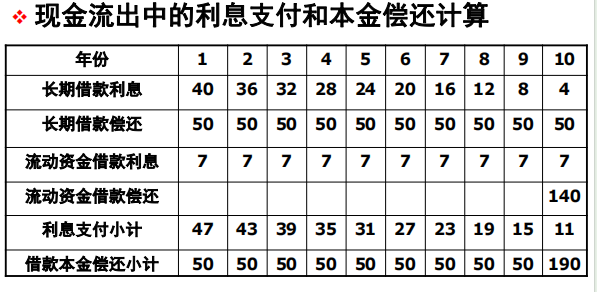
\includegraphics[width=0.75\linewidth]{image/生存能力分析2.png}
\end{figure}

\begin{figure}[H]
    \centering
    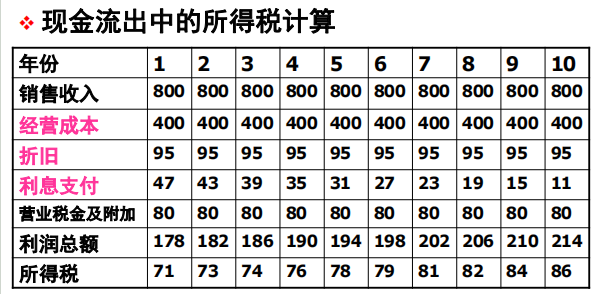
\includegraphics[width=0.75\linewidth]{image/生存能力分析3.png}
\end{figure}

\begin{figure}[H]
    \centering
    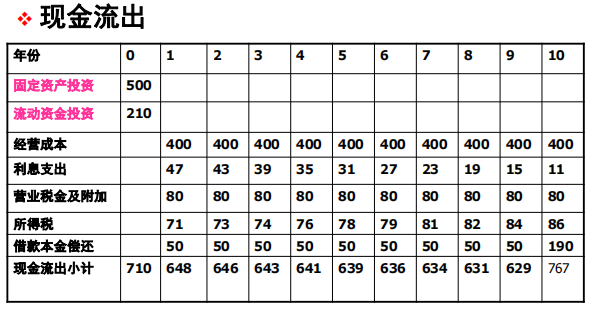
\includegraphics[width=0.75\linewidth]{image/生存能力分析4.png}
\end{figure}

\begin{figure}[H]
    \centering
    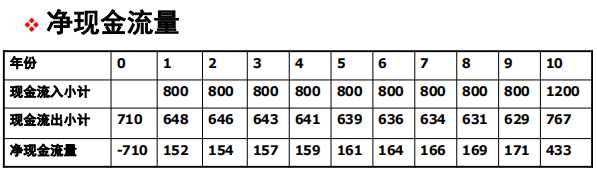
\includegraphics[width=0.75\linewidth]{image/生存能力分析5.png}
\end{figure}